%------------------------------------------------------------------------------
% Author(s):
% Varaun Ramgoolie
%
% Copyright:
%  Copyright (C) 2020 Brad Bachu, Arjun Mohammed, Varaun Ramgoolie, Nicholas Sammy
%
%  This file is part of Applied-Mathematics-Unit2 and is distributed under the
%  terms of the MIT License. See the LICENSE file for details.
%
%  Description:
%     Year: 2005 C
%     Module: 3
%     Question: 6
%------------------------------------------------------------------------------

%------------------------------------------------------------------------------
% 6 a
%------------------------------------------------------------------------------

\begin{subquestions}

We are given a ball that is launched at an angle to the horizontal.
	
\subquestion
	
\textbf{\textit{Sketch and Translate:}} \\ \\
We can refer to the diagram given in the question for our sketch. At the greatest height, we should note that the vertical velocity, $v_y$ will be 0.




\textbf{\textit{Simplify and Diagram:}} \\ \\ 
\addimage{../2005/figures/2005q6-Diagram1}{hhello}{Yes hi}
\begin{figure}[H] 
	\begin{center}
		\hspace{20pt}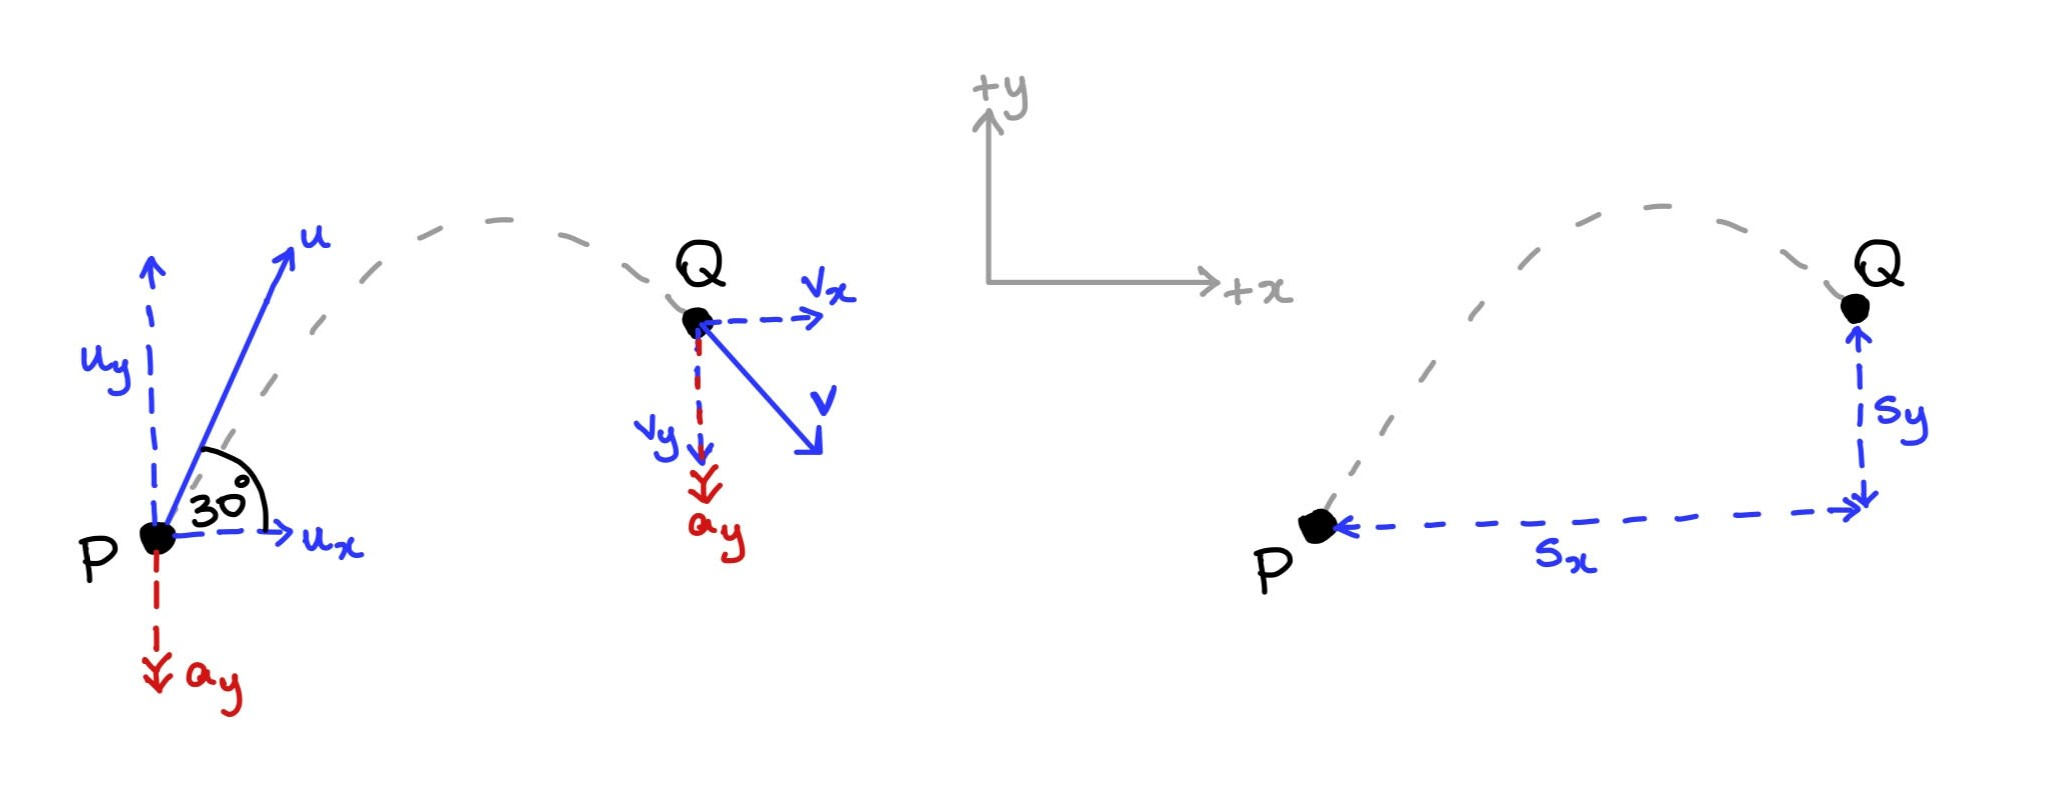
\includegraphics[scale=1.2]{../2005/figures/2005q6-Diagram1}
		\caption{\label{2005:q6:Diagram1} Motion of the ball. The left shows the velocity and acceleration of the ball, the right shows its displacement}
	\end{center}
\end{figure}

We will consider the ball to act as a point particle. Let us define the following:
\begin{itemize}
	\item $u$ is the initial velocity, $u=30$,
	\item $u_x$ is the initial horizontal velocity, $u_x = 30\cos(30)$,
	\item $u_y$ is the initial vertical velocity, $u_x = 30\sin(30)$
	\item $v_x$ is the final horizontal velocity,
	\item $v_y$ is the final vertical velocity,
	\item $a_x$ is the horizontal acceleration, $a_x=0$,
	\item $a_y$ is the vertical acceleration, $a_y=-g=-10$,
	\item $s_x$ is the horizontal displacement,
	\item $s_y$ is the vertical displacement,
	\item $t$ is the time after launch.
\end{itemize}
We can find the time taken to reach the maximum height by using our equations of motion.
	
	
	
	
\textbf{\textit{Represent Mathematically:}} \\ \\
At max height, we know that,
\begin{equation}
	v_y = 0 \,.
\end{equation}

We will find the time taken to reach the maximum height by using,
\begin{equation}
	v_y = u_y + a_yt \label{2005:q5:VEqn1} \,.
\end{equation}	
	



\textbf{\textit{Solve and Evaluate:}} \\ \\
Using \req{2005:q5:VEqn1}, we get that,
\begin{align}
	0 & = 30\sin(30) -10t \nn \\
	\implies t & = 1.5s \,. 
\end{align}

%------------------------------------------------------------------------------
% 6 b
%------------------------------------------------------------------------------

\subquestion 

\textbf{\textit{Simplify and Diagram:}} \\ \\
We can consider \rfig{2005:q6:Diagram1}. Again, we will use our equations of motion to find the greatest height reached. 




\textbf{\textit{Represent Mathematically:}} \\ \\
At max height, we know that,
\begin{equation}
	v_y = 0 \,.
\end{equation}

We will find the greatest height by using,
\begin{equation}
	v_y^2 = u_y^2 + 2a_ys_y \label{2005:q5:SEqn1} \,.
\end{equation}




\textbf{\textit{Solve and Evaluate:}} \\ \\
Using \req{2005:q5:SEqn1}, we get that,
\begin{align}
	0 & = (30\sin(30))^2 + 2(-10)(s_y) \nn \\
	\implies s_y & = \frac{900\sin^2(30)}{20} \nn \\
	             & = 11.25m \,.	
\end{align}

%------------------------------------------------------------------------------
% 6 c
%------------------------------------------------------------------------------

\subquestion 

\textbf{\textit{Sketch and Translate:}} \\ \\
We can consider \rfig{2005:q6:Sketch1}. At Q, we know that $s_y=10$.




\textbf{\textit{Sketch and Translate:}} \\ \\
We can consider \rfig{2005:q6:Diagram1}. We will use our equations of motion and find the times when $s_y=10$. We will take the value that is greater than 1.5s as we know, from the diagram in the question, that the ball reaches Q after it has attained its maximum height.




\textbf{\textit{Represent Mathematically:}} \\ \\
At Q, we know that,
\begin{equation}
	s_y=10 \,.
\end{equation}

To find the time taken to reach Q from P, we will use,
\begin{equation}
	s_y = u_yt + \frac{1}{2}a_yt^2 \label{2005:q6:SEqn2} \,.
\end{equation}




\textbf{\textit{Solve and Evaluate:}} \\ \\
Using \req{2005:q6:SEqn2}, we get,
\begin{align}
	10 & = 30\sin(30)t + \frac{1}{2}(-10)t^2 \nn \\
	5t^2-15t+10 & = 0 \nn \\
	(5t-5)(t-2) & = 0 \nn \\
	t & = 1, 2 \,.
\end{align}
From this, we get that it takes 2s for the ball to reach Q from P.

%------------------------------------------------------------------------------
% 6 d
%------------------------------------------------------------------------------

\subquestion 

\textbf{\textit{Simplify and Diagram:}} \\ \\
\begin{figure}[H] 
	\begin{center}
		\hspace{20pt}\includegraphics[scale=1.2]{../2005/figures/2005q6-Diagram2}
		\caption{\label{2005:q6:Diagram2} Ball at points P and Q}
	\end{center}
\end{figure}
We will define the following:
\begin{itemize}
	\item $v_P$ is the speed of the ball at P, $v_P=30$,
	\item $v_Q$ is the speed of the ball at Q,
	\item $m$ is the mass of the ball,
	\item $E_P$ is the total energy of the ball at P,
	\item $E_Q$ is the total energy of the ball at P.
	\item $h$ is the height at Q, $h=10$.
\end{itemize}
By the Principle of Conservation of Energy, we know that the total energy at point P is equal to the total energy at Q. At P, we will consider the height of the ball as 0. Therefore, the ball has only kinetic energy at P and has both kinetic and potential energy at Q.





\textbf{\textit{Represent Mathematically:}} \\ \\
The Total Energy of the ball at P is,
\begin{align}
	E_P & = KE \nn \\
	    & = \frac{1}{2}mv_P^2 \,.
\end{align}

The Total Energy of the ball at Q is,
\begin{align}
	E_P & = KE + PE \nn \\
        & = \frac{1}{2}mv_Q^2 + mgh \,.
\end{align}

By the Principle of Conservation of Energy, we get that,
\begin{align}
	E_P = E_Q \label{2005:q6:EEqn1} \,.
\end{align}




\textbf{\textit{Solve and Evaluate:}} \\ \\
Using \req{2005:q6:EEqn1}, we get that,
\begin{align}
	E_P & = E_Q \nn \\
	\frac{1}{2}mv_P^2 & = \frac{1}{2}mv_Q^2 + mgh \nn \\
	v_P^2 & = v_Q^2 +2gh \nn \\
	v_Q & = \sqrt{30^2 - 200} \nn \\
	    & = \sqrt{700} \,.
\end{align}
	
\end{subquestions}